% Options for packages loaded elsewhere
\PassOptionsToPackage{unicode}{hyperref}
\PassOptionsToPackage{hyphens}{url}
\documentclass[
  11pt,
]{article}
\usepackage{xcolor}
\usepackage[left=3cm,right=3cm,top=2.5cm,bottom=2.5cm]{geometry}
\usepackage{amsmath,amssymb}
\setcounter{secnumdepth}{5}
\usepackage{iftex}
\ifPDFTeX
  \usepackage[T1]{fontenc}
  \usepackage[utf8]{inputenc}
  \usepackage{textcomp} % provide euro and other symbols
\else % if luatex or xetex
  \usepackage{unicode-math} % this also loads fontspec
  \defaultfontfeatures{Scale=MatchLowercase}
  \defaultfontfeatures[\rmfamily]{Ligatures=TeX,Scale=1}
\fi
\usepackage{lmodern}
\ifPDFTeX\else
  % xetex/luatex font selection
\fi
% Use upquote if available, for straight quotes in verbatim environments
\IfFileExists{upquote.sty}{\usepackage{upquote}}{}
\IfFileExists{microtype.sty}{% use microtype if available
  \usepackage[]{microtype}
  \UseMicrotypeSet[protrusion]{basicmath} % disable protrusion for tt fonts
}{}
\usepackage{setspace}
\makeatletter
\@ifundefined{KOMAClassName}{% if non-KOMA class
  \IfFileExists{parskip.sty}{%
    \usepackage{parskip}
  }{% else
    \setlength{\parindent}{0pt}
    \setlength{\parskip}{6pt plus 2pt minus 1pt}}
}{% if KOMA class
  \KOMAoptions{parskip=half}}
\makeatother
\usepackage{longtable,booktabs,array}
\usepackage{caption}
\captionsetup[table]{skip=6pt}
\newcounter{none} % for unnumbered tables
\usepackage{calc} % for calculating minipage widths
% Correct order of tables after \paragraph or \subparagraph
\usepackage{etoolbox}
\makeatletter
\patchcmd\longtable{\par}{\if@noskipsec\mbox{}\fi\par}{}{}
\makeatother
% Allow footnotes in longtable head/foot
\IfFileExists{footnotehyper.sty}{\usepackage{footnotehyper}}{\usepackage{footnote}}
\makesavenoteenv{longtable}
\usepackage{graphicx}
\makeatletter
\newsavebox\pandoc@box
\newcommand*\pandocbounded[1]{% scales image to fit in text height/width
  \sbox\pandoc@box{#1}%
  \Gscale@div\@tempa{\textheight}{\dimexpr\ht\pandoc@box+\dp\pandoc@box\relax}%
  \Gscale@div\@tempb{\linewidth}{\wd\pandoc@box}%
  \ifdim\@tempb\p@<\@tempa\p@\let\@tempa\@tempb\fi% select the smaller of both
  \ifdim\@tempa\p@<\p@\scalebox{\@tempa}{\usebox\pandoc@box}%
  \else\usebox{\pandoc@box}%
  \fi%
}
% Set default figure placement to htbp
\def\fps@figure{htbp}
\makeatother
% definitions for citeproc citations
\NewDocumentCommand\citeproctext{}{}
\NewDocumentCommand\citeproc{mm}{%
  \begingroup\def\citeproctext{#2}\cite{#1}\endgroup}
\makeatletter
 % allow citations to break across lines
 \let\@cite@ofmt\@firstofone
 % avoid brackets around text for \cite:
 \def\@biblabel#1{}
 \def\@cite#1#2{{#1\if@tempswa , #2\fi}}
\makeatother
\newlength{\cslhangindent}
\setlength{\cslhangindent}{1.5em}
\newlength{\csllabelwidth}
\setlength{\csllabelwidth}{3em}
\newenvironment{CSLReferences}[2] % #1 hanging-indent, #2 entry-spacing
 {\begin{list}{}{%
  \setlength{\itemindent}{0pt}
  \setlength{\leftmargin}{0pt}
  \setlength{\parsep}{0pt}
  % turn on hanging indent if param 1 is 1
  \ifodd #1
   \setlength{\leftmargin}{\cslhangindent}
   \setlength{\itemindent}{-1\cslhangindent}
  \fi
  % set entry spacing
  \setlength{\itemsep}{#2\baselineskip}}}
 {\end{list}}
\usepackage{calc}
\newcommand{\CSLBlock}[1]{\hfill\break\parbox[t]{\linewidth}{\strut\ignorespaces#1\strut}}
\newcommand{\CSLLeftMargin}[1]{\parbox[t]{\csllabelwidth}{\strut#1\strut}}
\newcommand{\CSLRightInline}[1]{\parbox[t]{\linewidth - \csllabelwidth}{\strut#1\strut}}
\newcommand{\CSLIndent}[1]{\hspace{\cslhangindent}#1}
\setlength{\emergencystretch}{3em} % prevent overfull lines
\providecommand{\tightlist}{%
  \setlength{\itemsep}{0pt}\setlength{\parskip}{0pt}}
%% tools/stamp.tex
%% Provenance footer for PDFs rendered from this project.
%% Vendored by zzcollab; this file is not project-specific. The
%% footer prints the source document and the time of rendering.
%% The git version is defined here too, and so is available to a
%% project that wants it on the page, but it is left off the
%% default footer: it already names the staged copy in share/ and
%% appears in its manifest row. All values are supplied at render
%% time by tools/stamp-render.R, which writes a small generated
%% file that redefines the macros below. The \providecommand
%% defaults keep a bare LaTeX compile working when the document is
%% built without the wrapper.
\usepackage{fancyhdr}
\usepackage{xcolor}
\providecommand{\stampsource}{\detokenize{(source not recorded)}}
\providecommand{\stamptime}{(time not recorded)}
\providecommand{\stampversion}{\detokenize{(version not recorded)}}
\setlength{\footskip}{40pt}
\newcommand{\stampfootcontent}{%
  \footnotesize\color{gray}%
  \parbox[b]{\textwidth}{%
    \stamptime\hfill\thepage\\[2pt]%
    \ttfamily\raggedright\stampsource}}
\pagestyle{fancy}
\fancyhf{}
\fancyfoot[C]{\stampfootcontent}
\renewcommand{\headrulewidth}{0pt}
\renewcommand{\footrulewidth}{0.4pt}
%% The title page uses the `plain` page style; redefine it so the
%% stamp appears there too.
\fancypagestyle{plain}{%
  \fancyhf{}%
  \fancyfoot[C]{\stampfootcontent}%
  \renewcommand{\headrulewidth}{0pt}%
  \renewcommand{\footrulewidth}{0.4pt}}
\renewcommand{\stampsource}{\textasciitilde{}/\allowbreak{}prj/\allowbreak{}res/\allowbreak{}36-pmsimstats-ng/\allowbreak{}pmsimstats-ng/\allowbreak{}analysis/\allowbreak{}report/\allowbreak{}10-interaction-test-calibration/\allowbreak{}report.Rmd}
\renewcommand{\stamptime}{2026-10-29 10:06 PDT}
\renewcommand{\stampversion}{\detokenize{whitepapers-pre-series-121-g16c41f963-wip}}
\usepackage{amsmath}
\usepackage{amssymb}
\usepackage{booktabs}
\usepackage{longtable}
\usepackage{float}
\usepackage[mathlines]{lineno}
\linenumbers
\usepackage{booktabs}
\usepackage{longtable}
\usepackage{array}
\usepackage{multirow}
\usepackage{wrapfig}
\usepackage{float}
\usepackage{colortbl}
\usepackage{pdflscape}
\usepackage{tabu}
\usepackage{threeparttable}
\usepackage{threeparttablex}
\usepackage[normalem]{ulem}
\usepackage{makecell}
\usepackage{xcolor}
\usepackage{bookmark}
\IfFileExists{xurl.sty}{\usepackage{xurl}}{} % add URL line breaks if available
\urlstyle{same}
% fallback for those not using the hyperref driver hyperxmp:
\makeatletter
\@ifundefined{xmpquote}{\newcommand{\xmpquote}[1]{#1}}{}
\makeatother
\hypersetup{
  pdftitle={Type I calibration of a mixed-model interaction test in an aggregated N-of-1 simulation: mean-model misfit absorbed by REML and a cluster-robust remedy},
  pdfauthor={pmsimstats team},
  hidelinks,
  pdfcreator={LaTeX via pandoc}}

\title{Type I calibration of a mixed-model interaction test in an aggregated N-of-1 simulation: mean-model misfit absorbed by REML and a cluster-robust remedy}
\author{pmsimstats team}
\date{October 29, 2026}

\begin{document}
\maketitle

{
\setcounter{tocdepth}{2}
\tableofcontents
}
\setstretch{1.1}
\section*{Abstract}\label{abstract}
\addcontentsline{toc}{section}{Abstract}

\textbf{Background.} A linear mixed model with a random intercept and a
continuous-time autoregressive residual is a common analysis of an
aggregated N-of-1 trial. Its model-based Wald test of a
biomarker-by-drug interaction can be miscalibrated. We diagnosed why,
in one simulated design.

\textbf{Methods.} We simulated the null of the Hybrid design with
\(N = 70\) participants. We computed the population calibration ratio
\(\kappa\) exactly from the data-generating mean and covariance. We
crossed the mean model with the working covariance in a model ladder.
We compared model-based, CR2 cluster-robust and Kenward-Roger
inference, and generalized estimating equations.

\textbf{Results.} In the pre-correction run the
model-based standard error exceeded the empirical
standard deviation by 6.0 to
9.7 percent. The Type I error was
0.029 to 0.036 against 0.05. The analysis
mean, a linear trend plus a drug indicator, could not follow the
curved mean trajectories. Restricted maximum likelihood absorbed this
misfit into the variance parameters. Under the project's current
data-generating process the exact population \(\kappa\) of the
production model was
1.055 to 1.061 with the fitted mean. It was
1.006 with a correct mean and
1.005 to 1.008 with a free mean per visit. The calibrated
appearance of the random-intercept-only model was a cancellation of
two errors. In the pre-correction run the
CR2 test rejected at 0.045
to 0.049.

\textbf{Conclusions.} In this example the conservatism came mainly from
the mean model, not from the residual correlation. A visit-level mean
removed most of it. A CR2 standard error restored the size without
changing the model.

\section{Introduction}\label{introduction}

The linear mixed model is a standard tool for testing whether a
covariate moderates an effect in longitudinal data\textsuperscript{\citeproc{ref-laird1982}{1},\citeproc{ref-diggle2002}{2}}. The quantity of interest is a fixed-effect
interaction coefficient. Inference usually proceeds by a Wald test:
the estimate divided by a model-based standard error, referred to a
\(t\) distribution. The model-based standard error is consistent only
when the working model is correct. Two parts of the working model
matter. One is the within-participant covariance, the random effects
together with the residual correlation. The other is the mean model.

The consequences of a misspecified working covariance are well
established. The model-based standard error is then inconsistent, and
the sandwich estimator repairs it\textsuperscript{\citeproc{ref-eicker1967}{3}--\citeproc{ref-royall1986}{8}}.
Gurka, Edwards and Muller\textsuperscript{\citeproc{ref-gurka2011}{9}} proved that an underspecified
covariance biases mixed-model fixed-effect inference in large samples
as well as small ones. More participants do not remove the bias. Lu
and Mehrotra\textsuperscript{\citeproc{ref-lu2010}{10}} and Gosho et al.\textsuperscript{\citeproc{ref-gosho2017}{11}} compared the
sandwich, its small-sample corrections and the Kenward-Roger method
under misspecified covariance in longitudinal trials. Luke\textsuperscript{\citeproc{ref-luke2017}{12}} evaluated the Type I error of Kenward-Roger and
Satterthwaite tests in linear mixed models.

Less attention has gone to the mean model. When the fixed effects
cannot follow the true mean trajectory, the residuals carry a
systematic pattern. If that pattern is common to many participants,
restricted maximum likelihood (REML) treats it as covariance. The
variance parameters then absorb it, and the model-based standard error
of a fixed effect changes. This paper shows that this mechanism, not
the residual correlation structure, produced most of a conservative
interaction test in one simulation of aggregated N-of-1 trials.

The example comes from the pmsimstats-ng project. The project studies
power to detect biomarker-treatment interactions in aggregated N-of-1
trials under carryover\textsuperscript{\citeproc{ref-hendrickson2020}{13}}. Methods for combining
N-of-1 trials, including the choice of covariance, are reviewed by
Zucker, Ruthazer and Schmid\textsuperscript{\citeproc{ref-zucker2010}{14}} and by Araujo, Julious and
Senn\textsuperscript{\citeproc{ref-araujo2016}{15}}. The companion carryover paper\textsuperscript{\citeproc{ref-pmsimstats-paper02}{16}} recommends an analysis, G9, that uses a CR2
cluster-robust standard error. The companion test-procedure paper\textsuperscript{\citeproc{ref-pmsimstats-paper08}{17}} reports a conservative model-based mixed model
in a different design. The present paper supplies the diagnosis behind
that conservatism and behind the CR2 remedy.

We make three contributions, each confined to the example. First, we
compute the population calibration ratio \(\kappa\) exactly from the
data-generating mean and covariance. This separates the mean and
covariance contributions without Monte Carlo error. Second, we show
that the mean misfit, absorbed by REML, accounts for most of the
excess \(\kappa\), and that the apparent calibration of a
random-intercept-only model is a cancellation of errors. Third, we
report the CR2 remedy, Kenward-Roger and generalized estimating
equations on the same simulated datasets, with paired Monte Carlo
standard errors. Section 2 sets out the instruments. Section 3
describes the example. Section 4 reports the results. Section 5
discusses them.

\section{Diagnostic instruments}\label{diagnostic-instruments}

\subsection{A first-order decomposition of the rejection rate}\label{a-first-order-decomposition-of-the-rejection-rate}

Let \(\hat\theta\) estimate an interaction coefficient \(\theta\), with
model-based standard error \(\widehat{\mathrm{SE}}\) and denominator
degrees of freedom \(\nu\). The Wald test rejects \(H_0: \theta = 0\) at
level \(\alpha\) when \(|T| > t_{\nu, 1-\alpha/2}\), with
\(T = \hat\theta / \widehat{\mathrm{SE}}\). Write
\begin{equation}
\hat\theta = \mu + \sigma Z^{\star},
\qquad \mu = \mathbb E(\hat\theta), \quad
\sigma = \mathrm{SD}(\hat\theta).
\label{eq:decomp}
\end{equation}
Then \(Z^{\star}\) has mean zero and unit variance by construction. Let
\(\kappa = \mathbb E(\widehat{\mathrm{SE}})/\sigma\), the calibration
ratio. If the variability of \(\widehat{\mathrm{SE}}\) about its mean is
neglected,
\begin{equation}
T \approx \frac{1}{\kappa}\bigl(Z^{\star} + \delta\bigr),
\qquad \delta = \mu/\sigma,
\label{eq:wald}
\end{equation}
and
\begin{equation}
\alpha_{\mathrm{real}} \approx
\Pr\!\bigl(|Z^{\star} + \delta| > \kappa\, t_{\nu, 1-\alpha/2}\bigr).
\label{eq:alpha}
\end{equation}
Four quantities appear: the standardized bias \(\delta\), the scale
\(\kappa\), the degrees of freedom \(\nu\) and the law of \(Z^{\star}\).
When \(\hat\theta\) is approximately normal, \(\delta = 0\) and \(\nu\) is
large, the expression reduces to the closed form
\begin{equation}
\alpha_{\mathrm{real}} \approx 2\,\Phi\!\bigl(-\kappa\,
t_{\nu, 1-\alpha/2}\bigr).
\label{eq:closed}
\end{equation}

This is a first-order heuristic, not an exact or exhaustive
decomposition. Under the approximation, \(\mathrm{SD}(T) \approx
1/\kappa\) because \(\mathrm{SD}(Z^{\star}) = 1\). Any gap between
\(\mathrm{SD}(T)\) and \(1/\kappa\) comes from the variability of
\(\widehat{\mathrm{SE}}\) and from its dependence on \(\hat\theta\), which
the approximation discards. We therefore report a fifth diagnostic,
the coefficient of variation of the standard error,
\(\mathrm{CV}(\widehat{\mathrm{SE}})\). When it is large, the closed
form can fail even with \(\kappa = 1\). Section 4 shows two such cases.
The components are standard simulation performance measures: bias,
the ratio of model-based to empirical standard error, and the
rejection rate\textsuperscript{\citeproc{ref-morris2019simulation}{18}}. The bias \(\delta\) acts as the
noncentrality of a noncentral \(t\)\textsuperscript{\citeproc{ref-johnson1940noncentral}{19}}.
Approximate degrees of freedom \(\nu\) follow Satterthwaite\textsuperscript{\citeproc{ref-satterthwaite1946}{20}}, Welch\textsuperscript{\citeproc{ref-welch1947generalization}{21}} and Kenward
and Roger\textsuperscript{\citeproc{ref-kenward1997small}{22}}.

Two quantities are measured by simulation in addition to the rejection
rate. The degrees-of-freedom channel is checked by recomputing the
\(p\)-values against a normal reference. The shape of the null
distribution is checked by the empirical distribution function of the
\(p\)-values, which should be uniform.

\subsection{The calibration ratio under a misspecified mean and covariance}\label{the-calibration-ratio-under-a-misspecified-mean-and-covariance}

Let \(\hat\theta = \ell^\top\hat\beta\) for a contrast vector \(\ell\),
with \(\hat\beta\) the generalized least squares estimate under a
working covariance \(V_0\) and fixed-effects design \(X\). Clusters are
independent, so every cross-product below is a sum over participants.
The model-based variance is
\begin{equation}
v_0 = \ell^\top\bigl(X^\top V_0^{-1} X\bigr)^{-1}\ell .
\label{eq:v0}
\end{equation}
The true sampling variance is the sandwich
\begin{equation}
v = \ell^\top\bigl(X^\top V_0^{-1} X\bigr)^{-1}
\bigl(X^\top V_0^{-1}\, S\, V_0^{-1} X\bigr)
\bigl(X^\top V_0^{-1} X\bigr)^{-1}\ell
\label{eq:vsand}
\end{equation}\textsuperscript{\citeproc{ref-white1980}{5},\citeproc{ref-liang1986}{7},\citeproc{ref-boos2013}{23}}. Here \(S\) is the second moment of
the outcome about the fitted working mean. When the mean model is
correct, \(S = V\), the true covariance. When it is not,
\begin{equation}
S = V + r r^\top ,
\label{eq:vrr}
\end{equation}
where \(r\) is the misfit, the true mean minus the best-fitting working
mean. In a design where every participant on a randomization path
shares the same visit schedule, \(r\) is common to the participants of
the path. REML estimates the variance parameters of \(V_0\) by fitting
\(S\), not \(V\). A common misfit pattern therefore enters the estimated
variance components. The calibration ratio is \(\kappa^2 = v_0/v\),
with \(V_0\) at the pseudo-true values that minimize the
Kullback-Leibler criterion \(\log|V_0| + \mathrm{tr}(V_0^{-1} S)\)\textsuperscript{\citeproc{ref-white1982}{6},\citeproc{ref-patterson1971}{24},\citeproc{ref-harville1977}{25}}.

We compute \(\kappa\) exactly in this way from the data-generating
process (DGP). At the null the biomarker is independent of the
outcome with mean zero, so the information for the biomarker terms
separates from the rest. The computation needs only the per-path mean
and covariance of the outcome, which the DGP supplies in closed form.
It has no Monte Carlo error. It is a per-participant functional, so
it does not depend on the number of participants. It captures the
asymptotic calibration and excludes finite-sample REML terms by
construction. We validated it against the simulation in Section 4.

\subsection{A two-factor model ladder}\label{a-two-factor-model-ladder}

The ladder refits the same datasets under a mean model crossed with a
working covariance. The covariance factor has four rungs: ordinary
least squares (M0), a random intercept (M1), a continuous-time
first-order autoregressive residual alone (M2), and both (M3, the
production model). The mean factor has four levels: the fitted mean
of the analysis model, the fitted mean plus expectancy terms (the mean
structure of the project's F1 analysis), a free mean for each visit,
and a correct mean. The correct mean is a free mean for each
path-by-visit cell in simulation, and the true mean in the analytic
computation. Because every rung is fitted to the same data, the rungs
can be compared replicate by replicate.

\subsection{The sample-size gradient}\label{the-sample-size-gradient}

The analytic \(\kappa\) of Section 2.2 does not depend on the number of
participants. A simulation gradient in \(N\) therefore cannot show
whether the excess is asymptotic. That is settled by the analytic
computation. The gradient checks only for finite-sample terms in the
REML variance estimates, the terms that the Kenward-Roger correction
addresses\textsuperscript{\citeproc{ref-kenward1997small}{22},\citeproc{ref-kackar1984}{26}}. We report the slope of
the simulated \(\kappa\) on \(\log_2 N\) with a confidence interval.

\section{Worked example}\label{sec-example}

\subsection{Design and data-generating process}\label{design-and-data-generating-process}

Table \ref{tab:tab-ademp} summarizes the study in the ADEMP structure
of Morris, White and Crowther\textsuperscript{\citeproc{ref-morris2019simulation}{18}}. The design is
the Hybrid design: open-label titration, blinded discontinuation, then
a brief crossover. It has four randomization paths and eight visits,
at weeks 4, 8, 9, 10, 11, 12, 16 and 20. \(N = 70\) is the total across
paths, allocated 18, 18, 17 and 17. The outcome \(Y_{it}\) is a
baseline level minus three components: a natural-history component, a
placebo-response component whose standard deviation scales with the
design expectancy \(\eta_t\), and a drug-response component. Each
component follows a modified Gompertz mean curve and a first-order
autoregressive correlation in calendar weeks with \(\rho = 0.7\). The
components are non-negative reductions in symptom severity. An
increase in any component therefore lowers \(Y_{it}\), and interaction
coefficients are negative under the alternative.

Carryover acts on the drug-response mean after discontinuation, with a
half-life of \(t_{1/2} = 1\) week. The interaction is carried by the
correlation between the biomarker and the drug response, \(c_{bm}\)
(the covariance-moderation architecture of the companion DGP paper\textsuperscript{\citeproc{ref-pmsimstats-paper01}{27}}). At \(c_{bm} = 0\) the interaction is null, and
the mean-moderation and covariance-moderation architectures generate
identical data under a common seed (verified,
\texttt{check-null-architecture-equivalence.R}).

Two versions of the DGP appear in this paper. The \textbf{pre-correction
run} of 2026-05-20 used a cross-component correlation of
\(c_1 = 0.2\) at the same visit but \(c_\times = 0.1\) at different
visits, a mismatch documented in the project's driver audit. It also
used the original carryover rule, which compounds the decay. The
\textbf{extended DGP} of the companion DGP paper sets \(c_1 = c_\times = 0.2\),
lets carryover decay from the last on-drug mean, and stops on a
covariance matrix that is not positive definite. Every table caption
names the version that produced it. The analytic computation is
reported for both. No cell of either version needed a
positive-definiteness repair. The minimum eigenvalue of the
covariance matrix over the four paths is
0.104
for the pre-correction constants and
0.184
for the extended DGP at \(c_{bm} = 0\).

\begin{table}

\caption{\label{tab:tab-ademp}ADEMP summary of the simulation study.}
\centering
\begin{tabular}[t]{l>{\raggedright\arraybackslash}p{10cm}}
\toprule
Element & Content\\
\midrule
Aims & Explain the conservatism of the model-based interaction test and evaluate remedies.\\
Data-generating mechanisms & Hybrid design, N = 70, c\_bm = 0 (null) and 0.45 (alternative), half-life 1 week, rho = 0.7. Extended DGP and pre-correction run.\\
Estimand & theta, the biomarker-by-drug interaction coefficient. theta = 0 at the null.\\
Methods & E1, E2, E3 under M0 to M3 and four mean models. CR2 Satterthwaite, G9, F1. GEE with Liang-Zeger and Mancl-DeRouen sandwiches. Kenward-Roger on M2.\\
Performance measures & Rejection rate with MCSE and binomial test, kappa, CV of the SE, mean estimate with MCSE, paired differences between procedures.\\
\bottomrule
\end{tabular}
\end{table}

\subsection{The analysis model}\label{the-analysis-model}

The production analysis model is
\begin{equation}
Y_{it} = \beta_0 + \beta_B B_i + \beta_T w_t + \beta_D D^{\ast}_{it}
  + \theta\,B_i D^{\ast}_{it} + u_i + \varepsilon_{it},
\label{eq:lmm}
\end{equation}
with \(B_i\) the biomarker, drawn from \(\mathcal N(0, 1)\), \(w_t\) the
calendar week, \(u_i \sim \mathcal N(0, \sigma_u^2)\) a participant
random intercept, and \(\varepsilon_{it}\) a residual with
continuous-time first-order autoregressive correlation
\(\rho_a^{|w_t - w_s|}\) and variance \(\sigma_\varepsilon^2\). It is
fitted by REML with \texttt{nlme::lme}\textsuperscript{\citeproc{ref-pinheirobates2000}{28},\citeproc{ref-nlme3169}{29}}, with
\texttt{corCAR1(form\ =\ \textasciitilde{}t\ \textbar{}\ ptID)}. The drug term \(D^{\ast}_{it}\) defines
three specifications. Under E1 it is the binary drug state \(D_{it}\).
Under E2 it is the exposure-decayed indicator \(D_{bc,it}\) at the true
half-life. E3 uses \(D_{it}\) and adds the lagged just-off-drug
indicator \(L_{it}\). The interaction \(\theta\) is the coefficient of
\texttt{bm:Db} under E1 and E3 and of \texttt{bm:Dbc} under E2. This is the
historical analysis of the project, not its current recommendation.

In the codes of the companion carryover paper\textsuperscript{\citeproc{ref-pmsimstats-paper02}{16}},
E1 with model-based inference is G1 and with CR2 inference is G6. E2
at the true half-life is G3, and G8 with CR2. G9 is the recommended
analysis: E2 with the analysis half-life chosen by AIC over
\(\{0.25, 0.5, 1, 2\}\) weeks, a REML refit and a CR2 test. F1 adds the
design expectancy and its interaction with the biomarker,
\texttt{bm\ +\ t\ +\ Dbc\ +\ bm:Dbc\ +\ De\ +\ bm:De}, at a fixed analysis half-life
of 0.2 week, with a CR2 test.

\subsection{Replicates and Monte Carlo error}\label{replicates-and-monte-carlo-error}

The decomposition and the ladder used 5,000 null replicates, the CR2
and alternative-cell runs 3,000, generalized estimating equations
5,000, the Kenward-Roger check 2,000 and the gradient 1,500 per point.
All null-cell runs share one seed, so replicate \(i\) is the same
dataset in every run. Every comparison between procedures is
therefore paired. A rejection rate \(\hat\pi\) from \(n\) replicates has
Monte Carlo standard error (MCSE) \(\sqrt{\hat\pi(1-\hat\pi)/n}\). A
paired difference of rejection indicators has MCSE equal to the
standard deviation of the differences over \(\sqrt n\). The MCSE of
\(\kappa\) is approximated by \(\kappa/\sqrt{2(n-1)}\), which ignores the
variability of the mean standard error.

\section{Results}\label{results}

\subsection{The model-based test is conservative because its standard error is too large}\label{the-model-based-test-is-conservative-because-its-standard-error-is-too-large}

We fitted M3 to the primary null cell for E1, E2 and E3. Table
\ref{tab:tab-decomp} reports the decomposition. The model-based
standard error exceeded the empirical standard deviation of the
estimate, with \(\kappa\) = 1.068,
1.097 and 1.060 for E1, E2 and
E3. The MCSE of each \(\kappa\) is about
0.011. The Type I error was
0.033, 0.029 and 0.036,
each with MCSE about 0.0026. Each was below 0.05 by
an exact binomial test
(each \(p < 0.001\)).

\begin{table}
\centering
\caption{\label{tab:tab-decomp}First-order decomposition at the primary null cell (Hybrid, $N = 70$, $c_{bm} = 0$), production model M3 with the fitted mean. Pre-correction run of 2026-05-20 ($c_\times = 0.1$, original carryover rule). Fits that failed are excluded, not refitted without the residual correlation. Closed form is the closed-form size of Section 2.1 at the observed $\kappa$ and df.}
\centering
\resizebox{\ifdim\width>\linewidth\linewidth\else\width\fi}{!}{
\begin{tabular}[t]{lrlllllllll}
\toprule
Spec & n & Mean est. (MCSE) & $\kappa$ & CV(SE) & SD($T$) & Type I (MCSE) & Binom. $p$ & Type I, $z$ & Closed form & df\\
\midrule
E1 & 4968 & +0.031 (0.013) & 1.068 & 0.093 & 0.933 & 0.0330 (0.0025) & < 0.001 & 0.0340 & 0.036 & 487\\
E2 & 4960 & +0.039 (0.017) & 1.097 & 0.095 & 0.909 & 0.0294 (0.0024) & < 0.001 & 0.0296 & 0.031 & 487\\
E3 & 4960 & +0.033 (0.013) & 1.060 & 0.093 & 0.941 & 0.0357 (0.0026) & < 0.001 & 0.0359 & 0.037 & 486\\
\bottomrule
\end{tabular}}
\end{table}

The other first-order quantities did not produce the conservatism.
The degrees of freedom were about 487,
and a normal reference moved the Type I error by at most
0.0010. The closed form \eqref{eq:closed}
at the observed \(\kappa\) predicted 0.031 to
0.037. The observed range was 0.029 to
0.036. Each prediction exceeded its observed value, by
0.6 to
1.1 MCSE. The
three errors share a direction because the three specifications were
fitted to the same datasets. The linearization
\(\alpha_{\mathrm{real}} \approx 0.05 - 0.23(\kappa - 1)\), from the
derivative \(-2 z_{0.975}\varphi(z_{0.975}) = -0.229\) at \(\kappa = 1\),
is used only to state the elasticity
\(\mathrm{d}\log\alpha_{\mathrm{real}}/\mathrm{d}\log\kappa = -4.58\).
At \(\kappa\) = 1.097 it gives
0.028, against the closed form 0.031.

The mean estimate was +0.031 to
+0.039, 2.3 to
2.6 MCSE from zero. This is not a
property of the estimator. At \(c_{bm} = 0\) the biomarker is
independent of the outcome and symmetric about its mean. The model
contains the biomarker main effect and the drug main effect, so
replacing \(B_i\) by its reflection about the mean changes the sign of
\(\hat\theta\) and leaves the variance estimates unchanged. Hence
\(\mathbb E(\hat\theta) = 0\) exactly. The displacement is one chance
fluctuation. It recurs across specifications because they share
datasets: the E1 and E2 estimates have correlation
0.91.

The random-intercept standard deviation fell below 1 in
8.7 percent of E1 fits, at the boundary of the
parameter space, against a pseudo-true value of
9.85.
In the pre-correction run 32, 40 and 40 of the 5,000 fits for E1, E2 and E3 failed with the residual correlation and had been refitted without it. They are excluded here.

\begin{figure}

{\centering 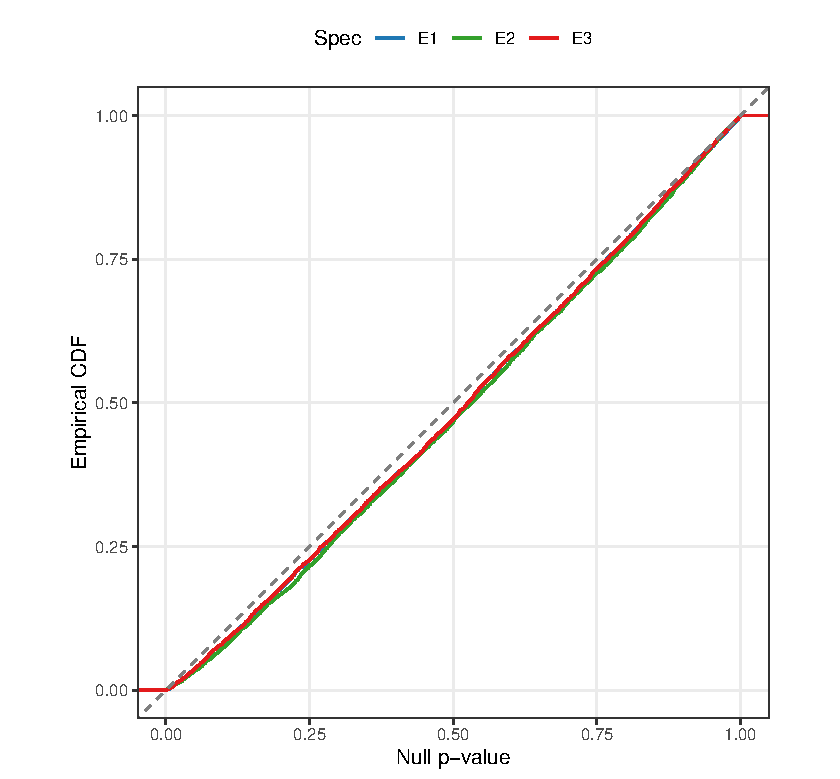
\includegraphics[width=0.6\linewidth]{report_files/figure-latex/fig-ecdf-1} 

}

\caption{Empirical distribution function of the null p-values of the model-based M3 test at the primary cell, against the Uniform(0,1) diagonal. The curves lie below the diagonal across the unit interval.}\label{fig:fig-ecdf}
\end{figure}

Figure \ref{fig:fig-ecdf} shows the null \(p\)-values. They lie below
the diagonal over the whole unit interval, as an inflated standard
error predicts.

\subsection{The excess comes mainly from the mean model}\label{the-excess-comes-mainly-from-the-mean-model}

We computed the population \(\kappa\) for every combination of mean
model and working covariance (Table \ref{tab:tab-analytic}). The
computation reproduced the simulation. For the
pre-correction DGP and E1 under
M3 it gave \(\kappa\) = 1.071 against
1.068 simulated, \(\rho_a\) =
0.659 against a simulated
median of 0.664, and \(\sigma_u\) =
9.85 against a median of
9.68. As a
check of the computation, a DGP whose outcome covariance is exactly a
random intercept plus an autoregressive residual returned \(\kappa\) =
1.000, \(\sigma_u\) =
10.00 and \(\rho_a\) =
0.70, the true values. That DGP holds the
placebo-response variance constant over visits.

\begin{longtable}[t]{lllllll}
\caption{\label{tab:tab-analytic}Population calibration ratio $\kappa$ computed exactly from the DGP mean and covariance, by mean model and working covariance (M0 independence, M1 random intercept, M2 autoregressive residual, M3 both). Pre-correction: $c_\times = 0.1$, original carryover rule. Extended: $c_\times = 0.2$, carryover decaying from the last on-drug mean. E3 is within 0.01 of E1 throughout and is in the data file.}\\
\toprule
DGP & Spec & Mean & M0 & M1 & M2 & M3\\
\midrule
Pre-correction & E1 & Fitted & 1.308 & 0.972 & 1.063 & 1.071\\
Pre-correction & E1 & Fitted + expectancy & 1.426 & 1.112 & 1.047 & 1.066\\
Pre-correction & E1 & Free per visit & 1.266 & 0.899 & 1.015 & 1.015\\
Pre-correction & E1 & Correct & 1.269 & 0.901 & 1.016 & 1.017\\
Pre-correction & E2 & Fitted & 1.269 & 0.949 & 1.132 & 1.082\\
\addlinespace
Pre-correction & E2 & Fitted + expectancy & 1.354 & 1.059 & 1.111 & 1.081\\
Pre-correction & E2 & Free per visit & 1.236 & 0.888 & 1.093 & 1.024\\
Pre-correction & E2 & Correct & 1.235 & 0.887 & 1.090 & 1.022\\
Extended & E1 & Fitted & 1.307 & 0.959 & 1.048 & 1.057\\
Extended & E1 & Fitted + expectancy & 1.442 & 1.116 & 1.038 & 1.053\\
\addlinespace
Extended & E1 & Free per visit & 1.266 & 0.886 & 0.999 & 1.005\\
Extended & E1 & Correct & 1.268 & 0.888 & 1.000 & 1.006\\
Extended & E2 & Fitted & 1.265 & 0.935 & 1.083 & 1.061\\
Extended & E2 & Fitted + expectancy & 1.362 & 1.058 & 1.070 & 1.058\\
Extended & E2 & Free per visit & 1.233 & 0.873 & 1.041 & 1.008\\
\addlinespace
Extended & E2 & Correct & 1.232 & 0.872 & 1.038 & 1.006\\
\bottomrule
\end{longtable}

The mean misfit was large. The standard deviation of the true mean of
the outcome over the eight visits of a path was
3.94
to 4.27
points. The fitted mean, a linear trend plus a drug term, left a
root-mean-square misfit of
4.18 to 4.41 points under M3. The
misfit is common to the participants of a path. REML absorbed it into
the variance parameters: under M3 the pseudo-true residual standard
deviation was 12.36 with
the fitted mean and 11.35
with the correct mean.

Under the extended DGP, M3 had \(\kappa\) = 1.055 to 1.061
with the fitted mean and 1.006 with the correct
mean, over E1 to E3. The covariance misspecification of M3 therefore
contributes about one percent at most, and the mean misfit the rest.
Under the pre-correction DGP the values were
1.064
to 1.082
and 1.017
to 1.022.
With a correct mean only the covariance differs between the two
versions, so the larger covariance share there came from the
mismatched cross-component constant. The remaining 0.006 under the
extended DGP comes from the placebo-response variance, which changes
with the design expectancy and so departs from a random intercept
plus an autoregressive residual. With that variance held constant the
computation returns \(\kappa = 1\), as reported above. A free mean for each visit, common to all
paths, removed nearly all of the excess: M3 gave
1.005 to 1.008. Adding the expectancy terms to the fitted
mean did not: M3 gave 1.050 to 1.058. The expectancy
covariate takes two values, so it cannot follow the curved
natural-history and drug-response means.

A paired simulation confirmed the analytic result. In
1,487 replicates of the null cell, with \(c_\times = 0.1\) and carryover
decaying from the last on-drug mean, M3 for E1 was fitted twice to
each dataset: once to \(Y_{it}\) and once to \(Y_{it}\) minus its true
path-by-visit mean. \(\kappa\) fell from 1.072 to
1.014, a paired difference of 0.057 with
bootstrap standard error 0.0027. The Type I error rose from
0.033 to 0.047, a paired difference of
+0.014 with MCSE 0.0031. This check was run by
the referee of an earlier draft (\texttt{diagnose-null-meanmisfit-referee.R}).

\begin{quote}\small\textbf{RESULTS-PENDING.} The correct-mean (oracle) arm under the extended DGP is in \texttt{diagnose-null-type1.R} and has not been run. Command, from the repository root, with thread variables set to 1: \texttt{bash analysis/scripts/carryover-sensitivity/run-paper10-refined.sh}. This driver alone costs about 0.7 CPU-hour (about 6 minutes on seven idle workers). The full set of drivers costs about 10 CPU-hours.\end{quote}

The ladder explains the random-intercept-only model (Table
\ref{tab:tab-ladder}). With the fitted mean, M1 was close to
calibrated. Its population \(\kappa\) was 0.935 to 0.959,
and in simulation M1 rejected at 0.049 for E1
and 0.055 for E2. With a correct mean its
population \(\kappa\) was 0.872 to 0.888. M1 would then be
anti-conservative, because it ignores the serial correlation. The
absorbed mean misfit raises its \(\kappa\) by a similar amount, and the
two errors cancel. The paired difference in Type I error between M1
and M3 for E1 was +0.017 (MCSE 0.0028).
Removing the residual correlation from M3 does not repair the test. It
trades one error for another.

\begin{table}
\centering
\caption{\label{tab:tab-ladder}Simulated ladder at the primary null cell. Pre-correction run of 2026-05-20 ($c_\times = 0.1$, original carryover rule). The same datasets are refitted under each row. The pre-correction run fitted only the fitted mean. Its M2 rung used \texttt{gls} with the optim optimizer and default tolerances, which did not reach the REML optimum (Section 5.2).}
\centering
\resizebox{\ifdim\width>\linewidth\linewidth\else\width\fi}{!}{
\begin{tabular}[t]{lllll}
\toprule
Mean & Model & Covariance & E1: $\kappa$ / Type I (MCSE) & E2: $\kappa$ / Type I (MCSE)\\
\midrule
Fitted & M0 & OLS & 1.323 / 0.0096 (0.0014) & 1.289 / 0.0116 (0.0015)\\
Fitted & M1 & Random intercept & 0.989 / 0.0492 (0.0031) & 0.972 / 0.0554 (0.0032)\\
Fitted & M2 & Autoregressive residual & 1.023 / 0.0434 (0.0029) & 1.070 / 0.0362 (0.0026)\\
Fitted & M3 & Both (production) & 1.068 / 0.0330 (0.0025) & 1.097 / 0.0294 (0.0024)\\
\bottomrule
\end{tabular}}
\end{table}

\begin{quote}\small\textbf{RESULTS-PENDING.} The simulated mean-model rungs (fitted mean plus expectancy, free mean per visit, free mean per path and visit) are in \texttt{diagnose-null-type1-stages46.R --stage 4} and have not been run. Table 3 gives their exact population values. Cost about 2.5 CPU-hours (about 20 minutes on seven idle workers). Command: as above.\end{quote}

\begin{figure}

{\centering 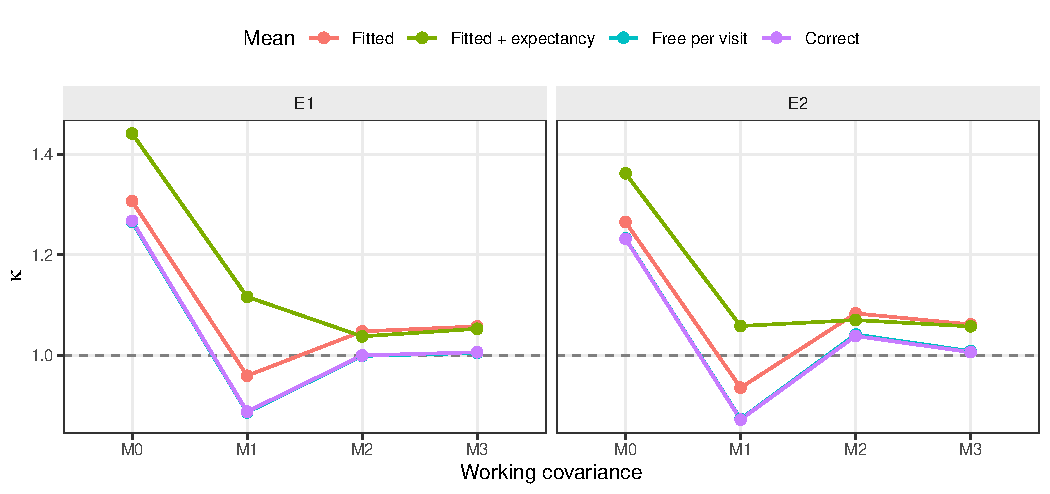
\includegraphics[width=1\linewidth]{report_files/figure-latex/fig-ladder-1} 

}

\caption{Population calibration ratio by working covariance and mean model, extended DGP, computed exactly. The dashed line marks calibration. With the fitted mean, M3 is conservative and M1 appears calibrated. With a correct or a per-visit mean, M3 is calibrated and M1 is anti-conservative.}\label{fig:fig-ladder}
\end{figure}

M0 had \(\kappa\) near 1.32. Ordinary least
squares charges a within-participant contrast with the
between-participant variance as well\textsuperscript{\citeproc{ref-neuhaus1998}{30}--\citeproc{ref-moulton1990}{32}}. The contrast is not purely
within participant, because the on-drug fraction differs by path, five
of eight visits on some paths and four of eight on others.

\subsection{The excess does not shrink with the number of participants}\label{the-excess-does-not-shrink-with-the-number-of-participants}

Table \ref{tab:tab-grad} reports M3 at \(N\) = 35, 70, 140 and 280. The
weighted slope of \(\kappa\) on \(\log_2 N\) was -0.003
(95 percent interval -0.020 to 0.014)
for E1, -0.008 (-0.026 to
0.009) for E2 and -0.003
(-0.019 to 0.014) for E3. The
intervals include zero. They are also wide enough to include a change
of 0.01 per doubling. The gradient therefore shows only that no large
finite-sample REML term is present. At \(N = 70\) the E1 and E3 sizes,
0.043 and 0.045, were within
1.3
MCSE of 0.05 at 1,500 replicates. The evidence that the excess is
asymptotic is the analytic computation of Section 4.2, which does not
depend on \(N\).

\begin{table}
\centering
\caption{\label{tab:tab-grad}Sample-size gradient, production model M3 with the fitted mean, 1,500 replicates per point. Pre-correction run of 2026-05-20 ($c_\times = 0.1$, original carryover rule). The MCSE of each $\kappa$ is about 0.02.}
\centering
\resizebox{\ifdim\width>\linewidth\linewidth\else\width\fi}{!}{
\begin{tabular}[t]{rlll}
\toprule
$N$ & E1: $\kappa$ / Type I (MCSE) & E2: $\kappa$ / Type I (MCSE) & E3: $\kappa$ / Type I (MCSE)\\
\midrule
35 & 1.072 / 0.038 (0.005) & 1.103 / 0.028 (0.004) & 1.064 / 0.039 (0.005)\\
70 & 1.056 / 0.043 (0.005) & 1.083 / 0.031 (0.004) & 1.050 / 0.045 (0.005)\\
140 & 1.086 / 0.041 (0.005) & 1.098 / 0.033 (0.005) & 1.079 / 0.042 (0.005)\\
280 & 1.052 / 0.037 (0.005) & 1.070 / 0.028 (0.004) & 1.046 / 0.035 (0.005)\\
\bottomrule
\end{tabular}}
\end{table}

\subsection{A cluster-robust standard error restores the size}\label{a-cluster-robust-standard-error-restores-the-size}

We replaced the model-based standard error of M3 by the CR2
bias-reduced cluster-robust standard error, clustered on participant,
with Satterthwaite degrees of freedom\textsuperscript{\citeproc{ref-satterthwaite1946}{20},\citeproc{ref-bell2002}{33},\citeproc{ref-pustejovsky2018}{34}}, computed with
\texttt{clubSandwich}\textsuperscript{\citeproc{ref-clubsandwich070}{35}}. Let \(\tilde e_i\) and \(\tilde X_i\)
be the residuals and design of participant \(i\) after the
generalized-least-squares transformation \(\hat V_0^{-1/2}\), and
\(H_{ii}\) the corresponding block of the hat matrix. A cluster-robust
variance is
\begin{equation}
\hat V_{\mathrm{CR}} = \bigl(\tilde X^\top \tilde X\bigr)^{-1}
  \Bigl(\textstyle\sum_i \tilde X_i^\top A_i\,\tilde e_i \tilde e_i^\top
  A_i \tilde X_i\Bigr)
  \bigl(\tilde X^\top \tilde X\bigr)^{-1}.
\label{eq:vcr}
\end{equation}
CR2 sets \(A_i = (I - H_{ii})^{-1/2}\), which makes
\(\hat V_{\mathrm{CR}}\) unbiased when the working model is correct\textsuperscript{\citeproc{ref-pustejovsky2018}{34},\citeproc{ref-mackinnon1985}{36}}. The jackknife choice
\(A_i = (I - H_{ii})^{-1}\) is the estimator of Mancl and DeRouen\textsuperscript{\citeproc{ref-mancl2001covariance}{37}} in the marginal setting. The Satterthwaite
degrees of freedom are \(\nu = (\sum_g \ell_g)^2 / \sum_g \ell_g^2\) in
the eigenvalues \(\ell_g\) of the matrix that defines the quadratic form\textsuperscript{\citeproc{ref-pustejovsky2018}{34}}. The point estimate and the model are unchanged.

\begin{table}
\centering
\caption{\label{tab:tab-cr2}CR2 remedy at the primary null cell, M3 with the fitted mean. Pre-correction run of 2026-05-20 ($c_\times = 0.1$, original carryover rule). Failed counts replicates in which the fit or the CR2 computation failed. They are excluded.}
\centering
\resizebox{\ifdim\width>\linewidth\linewidth\else\width\fi}{!}{
\begin{tabular}[t]{lrrllllllll}
\toprule
Spec & n & Failed & $\kappa$ model & $\kappa$ CR2 & CV(SE) CR2 & Type I model (MCSE) & Type I CR2 (MCSE) & Binom. $p$ CR2 & CR2 $-$ model (paired MCSE) & CR2 df (5th to 95th)\\
\midrule
E1 & 2980 & 20 & 1.062 & 0.978 & 0.168 & 0.0356 (0.0034) & 0.0483 (0.0039) & 0.705 & +0.0128 (0.0027) & 23.7 (17.4 to 29.9)\\
E2 & 2981 & 19 & 1.096 & 1.000 & 0.169 & 0.0288 (0.0031) & 0.0450 (0.0038) & 0.223 & +0.0161 (0.0029) & 23.7 (17.3 to 30.0)\\
E3 & 2976 & 24 & 1.053 & 0.976 & 0.168 & 0.0386 (0.0035) & 0.0491 (0.0040) & 0.866 & +0.0104 (0.0028) & 23.7 (17.3 to 29.9)\\
\bottomrule
\end{tabular}}
\end{table}

Table \ref{tab:tab-cr2} reports the result. The CR2 \(\kappa\) was
0.976 to
1.000. The CR2 Type
I error was 0.0483, 0.0450 and
0.0491, at \(z\) = -0.42,
-1.26 and
-0.24 from 0.05. The paired increase
over the model-based test was +0.013,
+0.016 and +0.010, with paired
MCSE 0.0027, 0.0029 and
0.0028. The CR2 computation failed in
20, 19 and 24 of the
3,000 replicates. These are excluded.

The closed form \eqref{eq:closed} does not hold for CR2. At the
observed CR2 \(\kappa\) and mean degrees of freedom it predicts
0.039 to
0.044. The
coefficient of variation of the CR2 standard error was
0.17, against 0.09 to 0.10
for the model-based one. The Satterthwaite reference absorbs that variability with
24 degrees of freedom, 5th to 95th
percentile 17 to
30, far below the model-based
487. The degrees of freedom reflect the
uneven leverage of participants on the interaction contrast. The paths
differ in their on-drug fraction, which is the likely source\textsuperscript{\citeproc{ref-carter2017}{38},\citeproc{ref-imbens2016}{39}}.

\begin{quote}\small\textbf{RESULTS-PENDING.} G9 (AIC half-life selection, REML refit, CR2) and F1 (expectancy terms, half-life 0.2 week, CR2) at the null cell are in \texttt{diagnose-null-type1-cr2.R} and have not been run. Cost with the CR2 arms about 1.5 CPU-hours (about 13 minutes on seven idle workers). Paper 02 reports G9 under its own grid.\end{quote}

\begin{figure}

{\centering 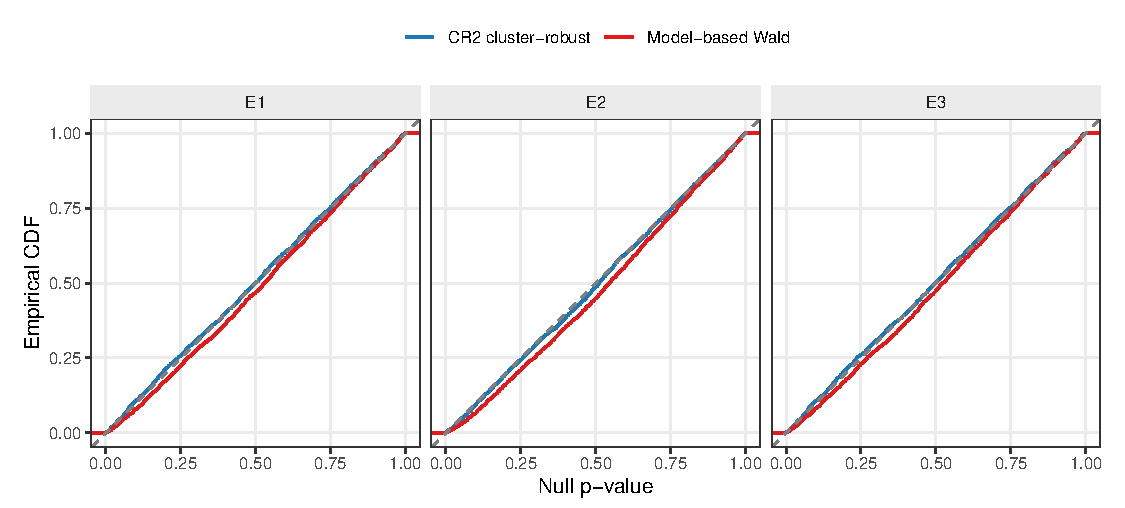
\includegraphics[width=1\linewidth]{report_files/figure-latex/fig-cr2-1} 

}

\caption{Null p-value distribution functions under the model-based and CR2 tests of M3, by specification. The model-based curves lie below the diagonal. The CR2 curves lie close to it.}\label{fig:fig-cr2}
\end{figure}

\subsection{The remedy at an alternative cell}\label{the-remedy-at-an-alternative-cell}

We repeated the comparison at \(c_{bm} = 0.45\) under the
covariance-moderation architecture, with the same design and \(N = 70\)
(Table \ref{tab:tab-alt}). The model-based \(\kappa\) was
1.119 to
1.152 and the CR2
\(\kappa\) 0.986 to
0.989. CR2 raised
power by +0.038, +0.034 and
+0.033 for E1, E2 and E3 (paired MCSE
0.0050, 0.0044 and
0.0050).

On the 2,932 replicates in which all three
specifications succeeded, the paired power advantage of E2 over E1
was +0.083 (MCSE 0.0060) under the model-based
test and +0.081 (MCSE 0.0058) under CR2. The
difference of these differences was -0.002 (MCSE
0.0059). The advantage of E2 over E3 was +0.086
(MCSE 0.0061) and +0.089 (MCSE 0.0059).
At this cell the recalibration raised power by a similar amount for
every specification and left their order unchanged. This is one cell.

\begin{table}
\centering
\caption{\label{tab:tab-alt}Alternative cell: covariance-moderation architecture, Hybrid, $N = 70$, $c_{bm} = 0.45$, half-life 1 week. Pre-correction run of 2026-05-20 ($c_\times = 0.1$, original carryover rule). Power is the rejection rate of M3 with the fitted mean.}
\centering
\resizebox{\ifdim\width>\linewidth\linewidth\else\width\fi}{!}{
\begin{tabular}[t]{lrlllll}
\toprule
Spec & n & $\kappa$ model & $\kappa$ CR2 & Power model (MCSE) & Power CR2 (MCSE) & CR2 $-$ model (paired MCSE)\\
\midrule
E1 & 2966 & 1.124 & 0.986 & 0.757 (0.0079) & 0.795 (0.0074) & +0.038 (0.0050)\\
E2 & 2981 & 1.152 & 0.988 & 0.843 (0.0067) & 0.878 (0.0060) & +0.034 (0.0044)\\
E3 & 2972 & 1.119 & 0.989 & 0.755 (0.0079) & 0.788 (0.0075) & +0.033 (0.0050)\\
\bottomrule
\end{tabular}}
\end{table}

\section{Discussion}\label{discussion}

\subsection{What the example shows}\label{what-the-example-shows}

In this example the model-based interaction test of the production
model was conservative. The main cause was the mean model. The fitted
mean, a linear trend plus a drug term, could not follow the curved
mean trajectories of the three components. REML treated the common
misfit as covariance, and the variance parameters grew. The
model-based standard error of the interaction grew with them. Under
the extended DGP the misspecified residual covariance contributed
about one percent of \(\kappa\). This revises the reading of an earlier
draft, which attributed the conservatism to the autoregressive
residual layer.

The revision changes the practical lesson. Removing the residual
correlation does not repair the test. It produces a model whose two
errors offset. A mean model that follows the visits does repair it.
In this design a free mean per visit brought the population \(\kappa\)
of M3 to 1.005 to 1.008. Expectancy terms alone did not.
The CR2 standard error repairs the size without changing the model.
It does not repair the cause. The two remedies can be combined. These
statements are confined to one DGP, one design and one estimand. That
a mean misfit absorbed by REML can make a mixed-model interaction test
conservative in other designs is a hypothesis, supported by the
\(V + rr^\top\) argument of Section 2.2 but not tested here.

The direction of the error depends on the model. M3 with the fitted
mean was conservative. M1 with a correct mean was anti-conservative.
The generalized estimating equations sandwich of Section 5.3 was
anti-conservative. Gurka, Edwards and Muller\textsuperscript{\citeproc{ref-gurka2011}{9}} showed that
an underspecified covariance can inflate the Type I error, and that
the bias does not shrink with the sample size. Our result is
compatible with theirs. Here the conservative direction arises
because the absorbed misfit inflates the variance parameters.

\subsection{Agreement with the companion test-procedure paper and Kenward-Roger}\label{agreement-with-the-companion-test-procedure-paper-and-kenward-roger}

The companion test-procedure paper\textsuperscript{\citeproc{ref-pmsimstats-paper08}{17}} reports a
model-based mixed model of the same class with \(\kappa\) of 1.10 to
1.16 and a size of 0.02 to 0.03, in a different design and DGP. It
classifies the conservatism as a calibration defect of the working
covariance, not of the degrees of freedom. It notes that Kenward-Roger
or Satterthwaite adjustments cannot repair a conservative test,
because they inflate the variance or lower the degrees of freedom. It
recommends CR2 inference. The present results agree on each point.
They refine the cause. The estimated working covariance is inflated,
and in this example the inflation comes from the mean misfit that
REML absorbs. We did not decompose the conservatism of that paper,
whose mean model includes expectancy terms but not a free mean per
visit.

Our empirical Kenward-Roger check is of the M2 rung, not of M3.
Kenward-Roger is available in R for marginal models through the
\texttt{mmrm} package\textsuperscript{\citeproc{ref-mmrm2026}{40}}, which does not fit a random intercept. SAS
PROC MIXED supports Kenward-Roger with a random intercept and a
spatial power residual. We did not run it. On the continuous-time
exponential covariance, Kenward-Roger changed the interaction standard
error by 0.07 percent on average (Table
\ref{tab:tab-kr}). On the unstructured covariance it changed it by
7.01 percent. With Kenward-Roger the unstructured
covariance still rejected at 0.0605
and 0.0620 for E1 and E3,
2.15 and
2.46 MCSE above 0.05. The
residual anti-conservatism agrees with Gosho et al.\textsuperscript{\citeproc{ref-gosho2017}{11}},
who found Kenward-Roger with an unstructured covariance close to
nominal only when the number of completers is large relative to the
number of visits.

\begin{longtable}[t]{llllll}
\caption{\label{tab:tab-kr}Kenward-Roger against Satterthwaite in \texttt{mmrm} at the primary null cell. Pre-correction run of 2026-05-20 ($c_\times = 0.1$, original carryover rule). The exponential fit has no random intercept: it is the M2 rung, not the production model M3. The Satterthwaite fit keeps the model-based covariance.}\\
\toprule
Covariance & Method & Spec & $\kappa$ & df & Type I (MCSE)\\
\midrule
Exponential (M2) & Kenward-Roger & E1 & 1.050 & 458 & 0.0400 (0.0044)\\
Exponential (M2) & Kenward-Roger & E2 & 1.138 & 514 & 0.0240 (0.0034)\\
Exponential (M2) & Kenward-Roger & E3 & 1.041 & 455 & 0.0430 (0.0045)\\
Exponential (M2) & Satterthwaite & E1 & 1.050 & 458 & 0.0400 (0.0044)\\
Exponential (M2) & Satterthwaite & E2 & 1.136 & 514 & 0.0240 (0.0034)\\
\addlinespace
Exponential (M2) & Satterthwaite & E3 & 1.040 & 455 & 0.0430 (0.0045)\\
Unstructured & Kenward-Roger & E1 & 0.951 & 172 & 0.0605 (0.0053)\\
Unstructured & Kenward-Roger & E2 & 0.965 & 148 & 0.0555 (0.0051)\\
Unstructured & Kenward-Roger & E3 & 0.948 & 171 & 0.0620 (0.0054)\\
Unstructured & Satterthwaite & E1 & 0.888 & 172 & 0.0785 (0.0060)\\
\addlinespace
Unstructured & Satterthwaite & E2 & 0.905 & 148 & 0.0710 (0.0057)\\
Unstructured & Satterthwaite & E3 & 0.884 & 171 & 0.0795 (0.0060)\\
\bottomrule
\end{longtable}

In the pre-correction run the \texttt{gls} fit of the M2 rung and the \texttt{mmrm}
exponential fit of nominally the same model disagreed, with a ratio of
mean standard errors of 1.004 for E1 and
0.981 for E2. The \texttt{gls} fit had used the \texttt{optim}
optimizer with default tolerances. With the \texttt{nlminb} optimizer and
tight tolerances, a check on 21 replicates of the extended DGP gave
standard errors that matched \texttt{mmrm} within a relative difference of
7.5e-06 in every one of
63 fits. The earlier M2 rung had not reached the REML
optimum. The corrected drivers use the tight settings.

\subsection{The marginal-model alternative}\label{the-marginal-model-alternative}

We fitted the generalized estimating equations counterpart of the
analysis model with \texttt{geepack}\textsuperscript{\citeproc{ref-halekoh2006}{41}}, Gaussian family and an
AR(1) working correlation (Table \ref{tab:tab-gee}). Two features
limit the comparison. First, \texttt{geepack} indexes the AR(1) lag by visit
order and ignores the irregular spacing of the Hybrid visits. We
checked that the reported standard error equals an inline sandwich
with order lags. A calendar-time working correlation is not available
in that package and was not evaluated. Second, in the pre-correction
run the Mancl-DeRouen standard error came from a separate refit with
\texttt{geesmv}\textsuperscript{\citeproc{ref-wang2016}{42}}. The corrected driver computes both standard errors from one
fit. In every case we report both standard errors against both
references, a normal one and \(t\) on \(K - p\) degrees of freedom, with
\(K\) participants and \(p\) fixed effects\textsuperscript{\citeproc{ref-li2015}{43}}.

\begin{table}
\centering
\caption{\label{tab:tab-gee}Generalized estimating equations at the primary null cell, AR(1) working correlation in visit order. Pre-correction run of 2026-05-20 ($c_\times = 0.1$, original carryover rule). LZ is the Liang-Zeger sandwich and MD the Mancl-DeRouen sandwich. Entries in the four rightmost rate columns are Type I error (MCSE). Relative efficiency is the variance of the M3 estimate over that of the GEE estimate on the same datasets.}
\centering
\resizebox{\ifdim\width>\linewidth\linewidth\else\width\fi}{!}{
\begin{tabular}[t]{lrlllllll}
\toprule
Spec & n & $\kappa$ LZ & $\kappa$ MD & LZ, $z$ & LZ, $t$ & MD, $z$ & MD, $t$ & Rel. eff.\\
\midrule
E1 & 5000 & 0.955 & 0.992 & 0.0684 (0.0036) & 0.0626 (0.0034) & 0.0590 (0.0033) & 0.0550 (0.0032) & 0.74\\
E2 & 5000 & 0.963 & 0.994 & 0.0674 (0.0035) & 0.0640 (0.0035) & 0.0624 (0.0034) & 0.0580 (0.0033) & 0.71\\
E3 & 5000 & 0.955 & 0.991 & 0.0686 (0.0036) & 0.0626 (0.0034) & 0.0588 (0.0033) & 0.0548 (0.0032) & 0.74\\
\bottomrule
\end{tabular}}
\end{table}

The Liang-Zeger sandwich gave \(\kappa\) of
0.955 to 0.963 and rejected at
0.067 to 0.069 with a normal reference.
The closed form \eqref{eq:closed} predicts 0.059 to
0.061 at those \(\kappa\), below the observed rates.
This is the second case where the first-order decomposition fails.
The sandwich standard error is variable and correlated with the
estimate\textsuperscript{\citeproc{ref-kauermann2001}{44}--\citeproc{ref-panwall2002}{46}}. The Mancl-DeRouen
correction with a \(t\) reference rejected at 0.0550,
0.0580 and 0.0548. For E2 this is
2.6 MCSE above 0.05 (binomial
\(p\) = 0.011). It is not calibrated at this
cluster count.

The GEE estimate was less efficient than the M3 estimate on the same
data. Its empirical standard deviation for E1 was
1.045 against 0.896, a relative
efficiency of 0.74. About
26 percent of the
information is lost. The marginal route is therefore not equivalent
to the conditional route with CR2 in this design. The CR2 test of M3
keeps the efficiency of the mixed-model estimate and comes closer to
the nominal size.

\subsection{Relation to the recommended analysis}\label{relation-to-the-recommended-analysis}

The CR2 tests evaluated here are G6 (E1) and G8 (E2) in the codes of
the companion carryover paper\textsuperscript{\citeproc{ref-pmsimstats-paper02}{16}}. That paper
recommends G9, which adds an AIC choice of the analysis half-life and
reports a measurable size increment from the selection step. The
present paper explains why the CR2 step is needed: the model-based
standard error of the historical analysis is inflated by the mean
misfit. The mean-model results suggest a further option, a free mean
per visit, which G9 does not use. Its power cost was not evaluated
here.

\subsection{Limitations}\label{limitations}

The study has one DGP, one design, one estimand and one alternative
cell. The analytic \(\kappa\) assumes equal allocation to paths,
whereas the simulation allocates 18, 18, 17 and 17, and it excludes
finite-sample terms by construction. The simulation tables come from
the pre-correction run unless a caption says otherwise.
Their magnitudes differ from the extended DGP by the amounts shown in Table 3: the population \(\kappa\) of M3 falls by about 0.01 to 0.02.
The parametric-bootstrap reference and the design-dependence analyses
of the examination plan (stages 4b and 5) were not run. The
examination plan expected M3 to be the well-specified member of the
ladder. The results show otherwise. Kenward-Roger was evaluated on M2
only. The power cost of a free mean per visit, and its behavior under
the alternative, were not evaluated. The ranking result at the
alternative rests on one cell. It should not be extended to
crossover designs or to the mean-moderation architecture without
evidence.

\section{Conclusions}\label{conclusions}

First, in this example the model-based Wald test of the interaction
in the production mixed model was conservative. Its standard error was
6.0 to 9.7 percent too
large and its size was 0.029 to 0.036.

Second, the main cause was the mean model. REML absorbed the misfit
of a linear trend plus a drug term into the variance parameters. With
a correct mean the population \(\kappa\) of M3 was
1.006.

Third, the apparent calibration of the random-intercept-only model
was a cancellation of two errors. It is not evidence that the
residual correlation should be dropped.

Fourth, the excess is asymptotic. The analytic \(\kappa\) does not depend
on the number of participants. Kenward-Roger changed the standard
error of the autoregressive M2 fit by about
0.07 percent. A degrees-of-freedom correction cannot
repair a conservative test.

Fifth, a CR2 cluster-robust standard error with Satterthwaite degrees
of freedom restored the size to within Monte Carlo error of 0.05 and
raised power at the alternative cell by a similar amount for each
specification. A free mean per visit removed most of the cause.

\section{Reproducibility}\label{reproducibility}

The drivers are in \texttt{analysis/scripts/carryover-sensitivity/}.
\texttt{paper10-common.R} holds the DGP settings of the corrected drivers:
\(c_1 = c_\times = 0.2\), carryover decaying from the last on-drug mean,
and a stop on a covariance matrix that is not positive definite. Each
run records the git commit and date in its output. The drivers are
\texttt{diagnose-kappa-analytic.R} (the population \(\kappa\)),
\texttt{diagnose-null-type1.R} (decomposition and correct-mean check),
\texttt{diagnose-null-type1-stages46.R} (ladder and gradient),
\texttt{diagnose-null-type1-cr2.R} (CR2, G9 and F1),
\texttt{diagnose-alt-cell-cr2.R} (alternative cell),
\texttt{diagnose-null-type1-gee.R} (generalized estimating equations),
\texttt{diagnose-null-type1-kr.R} (Kenward-Roger) and
\texttt{check-null-architecture-equivalence.R}. The script
\texttt{run-paper10-refined.sh} runs all of them with single-threaded linear
algebra and writes to \texttt{output/paper10-refined/}. The pre-correction
outputs of 2026-05-20 remain in \texttt{output/} for comparison. The
software versions were R
4.6.1, \texttt{nlme}
3.1-169, \texttt{clubSandwich} 0.7.0, \texttt{geepack} 1.3.13 and \texttt{mmrm} 0.3.17,
cited in Sections 3 to 5. The
examination plan that preceded the manuscript is retained as
\texttt{type1-examination-plan.md}.

\begin{quote}\small\textbf{RESULTS-PENDING.} The simulation tables of this draft come from the pre-correction run unless a caption says otherwise. The rerun under the extended DGP is prepared but not executed. Command, from the repository root: \texttt{bash analysis/scripts/carryover-sensitivity/run-paper10-refined.sh}. Estimated cost about 10 CPU-hours, 1.5 to 2 hours on seven idle workers. The manuscript switches each table automatically when the corresponding file holds its full replicate count. After the rerun, re-read the prose for qualitative statements that depend on the numbers.\end{quote}

\section*{Glossary}\label{glossary}
\addcontentsline{toc}{section}{Glossary}

\textbf{\(\kappa\).} The calibration ratio: the mean model-based standard
error divided by the empirical standard deviation of the estimates.
Above 1 the test is conservative.

\textbf{Population (pseudo-true) \(\kappa\).} \(\kappa\) computed exactly from
the DGP mean and covariance, with the working variance parameters at
the values REML converges to as the number of participants grows.

\textbf{Mean misfit.} The true mean of the outcome at a path and visit
minus the best-fitting mean of the analysis model.

\textbf{M0 to M3.} Working covariances: independence (ordinary least
squares), random intercept, continuous-time autoregressive residual
alone, and both. M3 is the production model.

\textbf{E1, E2, E3.} Drug terms of the analysis model. E1 is the binary
drug state. E2 is the exposure-decayed indicator at the true
half-life. E3 is the binary drug state plus a lagged just-off-drug
indicator.

\textbf{G1, G3, G6, G8, G9, F1.} Analysis codes of the companion carryover
paper. G1 and G3 are E1 and E2 with model-based inference. G6 and G8
are the same with CR2. G9 adds an AIC choice of the analysis
half-life. F1 adds the design expectancy and its interaction with the
biomarker at a fixed half-life of 0.2 week.

\textbf{Hybrid design.} Open-label titration, blinded discontinuation,
then a brief crossover, with four randomization paths.

\textbf{corCAR1.} The continuous-time first-order autoregressive residual
correlation of \texttt{nlme}, \(\rho_a^{|w_t - w_s|}\).

\textbf{\(c_{bm}\).} The correlation between the biomarker and the drug
response on drug, which carries the interaction in the
covariance-moderation architecture.

\textbf{\(c_1\), \(c_\times\).} Cross-component correlations at the same visit
and at different visits. The extended DGP sets both to 0.2. The
pre-correction run used \(c_\times = 0.1\). Code names \texttt{c.cf1t} and
\texttt{c.cfct}.

\textbf{Extended DGP.} The recommended data-generating process of the
companion DGP paper: separable AR(1) with \(\rho = 0.7\) and
\(c_1 = 0.2\), a biomarker-response correlation that decays after
discontinuation, carryover that decays from the last on-drug mean,
and a stop on matrices that are not positive definite. Code label
\texttt{refined}.

\textbf{Original carryover rule.} The carryover rule of the original DGP,
which applies the decay to the already-carried mean of the previous
visit and so compounds it.

\textbf{Pre-correction run.} The simulation outputs of 2026-05-20, made
with \(c_\times = 0.1\) and the original carryover rule.

\textbf{CV(SE).} The coefficient of variation of a standard error across
replicates.

\textbf{Paired MCSE.} The Monte Carlo standard error of a difference
between two procedures applied to the same datasets.

\section*{Abbreviations}\label{abbreviations}
\addcontentsline{toc}{section}{Abbreviations}

AIC, Akaike information criterion. CR2, bias-reduced cluster-robust
variance estimator of Bell and McCaffrey. DGP, data-generating
process. GEE, generalized estimating equations. KR, Kenward-Roger.
LZ, Liang-Zeger. MCSE, Monte Carlo standard error. MD, Mancl-DeRouen.
MMRM, mixed model for repeated measures. OLS, ordinary least squares.
REML, restricted maximum likelihood.

\section{References}\label{references}

\protect\phantomsection\label{refs}
\begin{CSLReferences}{0}{1}
\bibitem[\citeproctext]{ref-laird1982}
\CSLLeftMargin{1. }%
\CSLRightInline{Laird NM, Ware JH. Random-effects models for longitudinal data. \emph{Biometrics}. 1982;38(4):963-974. doi:\href{https://doi.org/10.2307/2529876}{10.2307/2529876}}

\bibitem[\citeproctext]{ref-diggle2002}
\CSLLeftMargin{2. }%
\CSLRightInline{Diggle PJ, Heagerty P, Liang KY, Zeger SL. \emph{Analysis of Longitudinal Data}. 2nd ed. Oxford University Press; 2002.}

\bibitem[\citeproctext]{ref-eicker1967}
\CSLLeftMargin{3. }%
\CSLRightInline{Eicker F. Limit theorems for regressions with unequal and dependent errors. In: \emph{Proceedings of the Fifth {Berkeley} Symposium on Mathematical Statistics and Probability, Volume 1}. University of California Press; 1967:59-82.}

\bibitem[\citeproctext]{ref-huber1967}
\CSLLeftMargin{4. }%
\CSLRightInline{Huber PJ. The behavior of maximum likelihood estimates under nonstandard conditions. In: \emph{Proceedings of the Fifth {Berkeley} Symposium on Mathematical Statistics and Probability, Volume 1}. University of California Press; 1967:221-233.}

\bibitem[\citeproctext]{ref-white1980}
\CSLLeftMargin{5. }%
\CSLRightInline{White H. A heteroskedasticity-consistent covariance matrix estimator and a direct test for heteroskedasticity. \emph{Econometrica}. 1980;48(4):817-838. doi:\href{https://doi.org/10.2307/1912934}{10.2307/1912934}}

\bibitem[\citeproctext]{ref-white1982}
\CSLLeftMargin{6. }%
\CSLRightInline{White H. Maximum likelihood estimation of misspecified models. \emph{Econometrica}. 1982;50(1):1-25.}

\bibitem[\citeproctext]{ref-liang1986}
\CSLLeftMargin{7. }%
\CSLRightInline{Liang KY, Zeger SL. Longitudinal data analysis using generalized linear models. \emph{Biometrika}. 1986;73(1):13-22. doi:\href{https://doi.org/10.1093/biomet/73.1.13}{10.1093/biomet/73.1.13}}

\bibitem[\citeproctext]{ref-royall1986}
\CSLLeftMargin{8. }%
\CSLRightInline{Royall RM. Model robust confidence intervals using maximum likelihood estimators. \emph{International Statistical Review}. 1986;54(2):221-226. doi:\href{https://doi.org/10.2307/1403146}{10.2307/1403146}}

\bibitem[\citeproctext]{ref-gurka2011}
\CSLLeftMargin{9. }%
\CSLRightInline{Gurka MJ, Edwards LJ, Muller KE. Avoiding bias in mixed model inference for fixed effects. \emph{Statistics in Medicine}. 2011;30(22):2696-2707. doi:\href{https://doi.org/10.1002/sim.4293}{10.1002/sim.4293}}

\bibitem[\citeproctext]{ref-lu2010}
\CSLLeftMargin{10. }%
\CSLRightInline{Lu K, Mehrotra DV. Specification of covariance structure in longitudinal data analysis for randomized clinical trials. \emph{Statistics in Medicine}. 2010;29(4):474-488. doi:\href{https://doi.org/10.1002/sim.3820}{10.1002/sim.3820}}

\bibitem[\citeproctext]{ref-gosho2017}
\CSLLeftMargin{11. }%
\CSLRightInline{Gosho M, Hirakawa A, Noma H, Maruo K, Sato Y. Comparison of bias-corrected covariance estimators for {MMRM} analysis in longitudinal data with dropouts. \emph{Statistical Methods in Medical Research}. 2017;26(5):2389-2406. doi:\href{https://doi.org/10.1177/0962280215597938}{10.1177/0962280215597938}}

\bibitem[\citeproctext]{ref-luke2017}
\CSLLeftMargin{12. }%
\CSLRightInline{Luke SG. Evaluating significance in linear mixed-effects models in {R}. \emph{Behavior Research Methods}. 2017;49(4):1494-1502. doi:\href{https://doi.org/10.3758/s13428-016-0809-y}{10.3758/s13428-016-0809-y}}

\bibitem[\citeproctext]{ref-hendrickson2020}
\CSLLeftMargin{13. }%
\CSLRightInline{Hendrickson RC, Thomas RG, Schork NJ, Raskind MA. Optimizing aggregated {N}-of-1 trial designs for predictive biomarker validation: Statistical methods and theoretical findings. \emph{Frontiers in Digital Health}. 2020;2:13. doi:\href{https://doi.org/10.3389/fdgth.2020.00013}{10.3389/fdgth.2020.00013}}

\bibitem[\citeproctext]{ref-zucker2010}
\CSLLeftMargin{14. }%
\CSLRightInline{Zucker DR, Ruthazer R, Schmid CH. Individual ({N}-of-1) trials can be combined to give population comparative treatment effect estimates: Methodologic considerations. \emph{Journal of Clinical Epidemiology}. 2010;63(12):1312-1323. doi:\href{https://doi.org/10.1016/j.jclinepi.2010.04.020}{10.1016/j.jclinepi.2010.04.020}}

\bibitem[\citeproctext]{ref-araujo2016}
\CSLLeftMargin{15. }%
\CSLRightInline{Araujo A, Julious S, Senn S. Understanding variation in sets of {N}-of-1 trials. \emph{PLoS One}. 2016;11(12):e0167167. doi:\href{https://doi.org/10.1371/journal.pone.0167167}{10.1371/journal.pone.0167167}}

\bibitem[\citeproctext]{ref-pmsimstats-paper02}
\CSLLeftMargin{16. }%
\CSLRightInline{{pmsimstats team}. Carryover representation and inference for biomarker-treatment interaction tests in aggregated {N}-of-1 trials under covariance moderation: A staged simulation study and a recommended analysis for the {Hybrid} design. Published online 2026.}

\bibitem[\citeproctext]{ref-pmsimstats-paper08}
\CSLLeftMargin{17. }%
\CSLRightInline{{pmsimstats team}. Test-procedure choice for the biomarker-treatment interaction in aggregated {N}-of-1 trials: Dichotomization, classical {RM-ANOVA}, mixed-effects, and generalized estimating equations. Published online 2026.}

\bibitem[\citeproctext]{ref-morris2019simulation}
\CSLLeftMargin{18. }%
\CSLRightInline{Morris TP, White IR, Crowther MJ. Using simulation studies to evaluate statistical methods. \emph{Statistics in Medicine}. 2019;38(11):2074-2102. doi:\href{https://doi.org/10.1002/sim.8086}{10.1002/sim.8086}}

\bibitem[\citeproctext]{ref-johnson1940noncentral}
\CSLLeftMargin{19. }%
\CSLRightInline{Johnson NL, Welch BL. Applications of the non-central \(t\)-distribution. \emph{Biometrika}. 1940;31(3--4):362-389.}

\bibitem[\citeproctext]{ref-satterthwaite1946}
\CSLLeftMargin{20. }%
\CSLRightInline{Satterthwaite FE. An approximate distribution of estimates of variance components. \emph{Biometrics Bulletin}. 1946;2(6):110-114. doi:\href{https://doi.org/10.2307/3002019}{10.2307/3002019}}

\bibitem[\citeproctext]{ref-welch1947generalization}
\CSLLeftMargin{21. }%
\CSLRightInline{Welch BL. The generalization of {{``Student's''}} problem when several different population variances are involved. \emph{Biometrika}. 1947;34(1--2):28-35.}

\bibitem[\citeproctext]{ref-kenward1997small}
\CSLLeftMargin{22. }%
\CSLRightInline{Kenward MG, Roger JH. Small sample inference for fixed effects from restricted maximum likelihood. \emph{Biometrics}. 1997;53(3):983-997. doi:\href{https://doi.org/10.2307/2533558}{10.2307/2533558}}

\bibitem[\citeproctext]{ref-boos2013}
\CSLLeftMargin{23. }%
\CSLRightInline{Boos DD, Stefanski LA. \emph{Essential Statistical Inference: Theory and Methods}. Springer; 2013.}

\bibitem[\citeproctext]{ref-patterson1971}
\CSLLeftMargin{24. }%
\CSLRightInline{Patterson HD, Thompson R. Recovery of inter-block information when block sizes are unequal. \emph{Biometrika}. 1971;58(3):545-554.}

\bibitem[\citeproctext]{ref-harville1977}
\CSLLeftMargin{25. }%
\CSLRightInline{Harville DA. Maximum likelihood approaches to variance component estimation and to related problems. \emph{Journal of the American Statistical Association}. 1977;72(358):320-338.}

\bibitem[\citeproctext]{ref-kackar1984}
\CSLLeftMargin{26. }%
\CSLRightInline{Kackar RN, Harville DA. Approximations for standard errors of estimators of fixed and random effects in mixed linear models. \emph{Journal of the American Statistical Association}. 1984;79(388):853-862. doi:\href{https://doi.org/10.1080/01621459.1984.10477102}{10.1080/01621459.1984.10477102}}

\bibitem[\citeproctext]{ref-pmsimstats-paper01}
\CSLLeftMargin{27. }%
\CSLRightInline{{pmsimstats team}. Simulating predictive-biomarker interactions in aggregated {N}-of-1 trials: An extended data-generating process building on {Hendrickson} et al. Published online 2026.}

\bibitem[\citeproctext]{ref-pinheirobates2000}
\CSLLeftMargin{28. }%
\CSLRightInline{Pinheiro JC, Bates DM. \emph{Mixed-Effects Models in {S} and {S-PLUS}}. Springer; 2000.}

\bibitem[\citeproctext]{ref-nlme3169}
\CSLLeftMargin{29. }%
\CSLRightInline{Pinheiro J, Bates D, R Core Team. \emph{Nlme: Linear and Nonlinear Mixed Effects Models}.; 2026. \url{https://CRAN.R-project.org/package=nlme}}

\bibitem[\citeproctext]{ref-neuhaus1998}
\CSLLeftMargin{30. }%
\CSLRightInline{Neuhaus JM, Kalbfleisch JD. Between- and within-cluster covariate effects in the analysis of clustered data. \emph{Biometrics}. 1998;54(2):638-645.}

\bibitem[\citeproctext]{ref-scott1982}
\CSLLeftMargin{31. }%
\CSLRightInline{Scott AJ, Holt D. The effect of two-stage sampling on ordinary least squares methods. \emph{Journal of the American Statistical Association}. 1982;77(380):848-854.}

\bibitem[\citeproctext]{ref-moulton1990}
\CSLLeftMargin{32. }%
\CSLRightInline{Moulton BR. An illustration of a pitfall in estimating the effects of aggregate variables on micro units. \emph{The Review of Economics and Statistics}. 1990;72(2):334-338. doi:\href{https://doi.org/10.2307/2109724}{10.2307/2109724}}

\bibitem[\citeproctext]{ref-bell2002}
\CSLLeftMargin{33. }%
\CSLRightInline{Bell RM, McCaffrey DF. Bias reduction in standard errors for linear regression with multi-stage samples. \emph{Survey Methodology}. 2002;28(2):169-181.}

\bibitem[\citeproctext]{ref-pustejovsky2018}
\CSLLeftMargin{34. }%
\CSLRightInline{Pustejovsky JE, Tipton E. Small-sample methods for cluster-robust variance estimation and hypothesis testing in fixed effects models. \emph{Journal of Business \& Economic Statistics}. 2018;36(4):672-683. doi:\href{https://doi.org/10.1080/07350015.2016.1247004}{10.1080/07350015.2016.1247004}}

\bibitem[\citeproctext]{ref-clubsandwich070}
\CSLLeftMargin{35. }%
\CSLRightInline{Pustejovsky JE. \emph{clubSandwich: Cluster-Robust (Sandwich) Variance Estimators with Small-Sample Corrections}.; 2026. \url{https://CRAN.R-project.org/package=clubSandwich}}

\bibitem[\citeproctext]{ref-mackinnon1985}
\CSLLeftMargin{36. }%
\CSLRightInline{MacKinnon JG, White H. Some heteroskedasticity-consistent covariance matrix estimators with improved finite sample properties. \emph{Journal of Econometrics}. 1985;29(3):305-325. doi:\href{https://doi.org/10.1016/0304-4076(85)90158-7}{10.1016/0304-4076(85)90158-7}}

\bibitem[\citeproctext]{ref-mancl2001covariance}
\CSLLeftMargin{37. }%
\CSLRightInline{Mancl LA, DeRouen TA. A covariance estimator for {GEE} with improved small-sample properties. \emph{Biometrics}. 2001;57(1):126-134. doi:\href{https://doi.org/10.1111/j.0006-341X.2001.00126.x}{10.1111/j.0006-341X.2001.00126.x}}

\bibitem[\citeproctext]{ref-carter2017}
\CSLLeftMargin{38. }%
\CSLRightInline{Carter AV, Schnepel KT, Steigerwald DG. Asymptotic behavior of a \(t\)-test robust to cluster heterogeneity. \emph{The Review of Economics and Statistics}. 2017;99(4):698-709.}

\bibitem[\citeproctext]{ref-imbens2016}
\CSLLeftMargin{39. }%
\CSLRightInline{Imbens GW, Kolesár M. Robust standard errors in small samples: Some practical advice. \emph{The Review of Economics and Statistics}. 2016;98(4):701-712. doi:\href{https://doi.org/10.1162/REST_a_00552}{10.1162/REST\_a\_00552}}

\bibitem[\citeproctext]{ref-mmrm2026}
\CSLLeftMargin{40. }%
\CSLRightInline{Sabanes Bove D, Li L, Dedic J, et al. \emph{Mmrm: Mixed Models for Repeated Measures}.; 2026. doi:\href{https://doi.org/10.32614/CRAN.package.mmrm}{10.32614/CRAN.package.mmrm}}

\bibitem[\citeproctext]{ref-halekoh2006}
\CSLLeftMargin{41. }%
\CSLRightInline{Halekoh U, Højsgaard S, Yan J. The {R} package geepack for generalized estimating equations. \emph{Journal of Statistical Software}. 2006;15(2):1-11. doi:\href{https://doi.org/10.18637/jss.v015.i02}{10.18637/jss.v015.i02}}

\bibitem[\citeproctext]{ref-wang2016}
\CSLLeftMargin{42. }%
\CSLRightInline{Wang M, Kong L, Li Z, Zhang L. Covariance estimators for generalized estimating equations ({GEE}) in longitudinal analysis with small samples. \emph{Statistics in Medicine}. 2016;35(10):1706-1721. doi:\href{https://doi.org/10.1002/sim.6817}{10.1002/sim.6817}}

\bibitem[\citeproctext]{ref-li2015}
\CSLLeftMargin{43. }%
\CSLRightInline{Li P, Redden DT. Small sample performance of bias-corrected sandwich estimators for cluster-randomized trials with binary outcomes. \emph{Statistics in Medicine}. 2015;34(2):281-296. doi:\href{https://doi.org/10.1002/sim.6344}{10.1002/sim.6344}}

\bibitem[\citeproctext]{ref-kauermann2001}
\CSLLeftMargin{44. }%
\CSLRightInline{Kauermann G, Carroll RJ. A note on the efficiency of sandwich covariance matrix estimation. \emph{Journal of the American Statistical Association}. 2001;96(456):1387-1396.}

\bibitem[\citeproctext]{ref-fay2001}
\CSLLeftMargin{45. }%
\CSLRightInline{Fay MP, Graubard BI. Small-sample adjustments for {Wald}-type tests using sandwich estimators. \emph{Biometrics}. 2001;57(4):1198-1206. doi:\href{https://doi.org/10.1111/j.0006-341x.2001.01198.x}{10.1111/j.0006-341x.2001.01198.x}}

\bibitem[\citeproctext]{ref-panwall2002}
\CSLLeftMargin{46. }%
\CSLRightInline{Pan W, Wall MM. Small-sample adjustments in using the sandwich variance estimator in generalized estimating equations. \emph{Statistics in Medicine}. 2002;21(10):1429-1441. doi:\href{https://doi.org/10.1002/sim.1142}{10.1002/sim.1142}}

\end{CSLReferences}

\end{document}
